\documentclass{beamer}
\usepackage[utf8]{inputenc}
%\usepackage{program}

\usepackage{tikz}
\usepackage{xspace}
\usetikzlibrary{arrows,positioning}

%\usepackage[czech]{babel}

% \usepackage{graphicx}
% \usepackage{color}
% \usepackage{listings}

\beamertemplatenavigationsymbolsempty
\usetheme{Frankfurt}
\setbeamercolor{title}{bg=green!40!black}
\setbeamercolor{frametitle}{bg=green!40!black}
\setbeamercolor{block title}{bg=green!45!black}
\setbeamercolor{block title alerted}{bg=yellow!50!red!80!black}
\setbeamercolor{alerted}{bg=yellow!50!red!80!black}
\setbeamertemplate{headline}{}

\newcommand{\tit}{\divine-2.5.2 Overview}
\newcommand{\divine}{\textsc{Di\hspace*{-1pt}V\hspace*{-1pt}inE}\xspace} 

\title{\divine -- Parallel LTL Model Checker}
\author{\Large\alert{\tit}}
\date{}

\setbeamertemplate{footline}{\tit \hfill str. \insertframenumber/\inserttotalframenumber}


\newcommand{\mysection}[1]{
\section{#1}
\frame{\frametitle{Sekce}
  \begin{center}
    \alert{\LARGE #1}
  \end{center}
}}

\begin{document}


\maketitle

\frame{\frametitle{\divine}
\textbf{\divine}
\begin{itemize}
\item LTL Model Checker
\item Explicit state
\item Automata-based approach
\end{itemize}
\bigskip
\textbf{Unique features}
\begin{itemize}
\item Non-DFS-based LTL MC algorithms
\item Parallel \& Distributed-memory processing
\item Parallel POR for LTL via Topological Sort Proviso
\end{itemize}
}

\frame{\frametitle{Getting \divine}
\textbf{Stable release}
\begin{itemize}
\item \url{http://divine.fi.muni.cz/}
\item Latest version -- 2.5.2
\item Windows pre-compiled version -- 2.5.0
\end{itemize}
\bigskip

\textbf{DARCS repository}
\begin{itemize}
\item darcs get http://divine.fi.muni.cz/darcs/mainline divine-2.x
\end{itemize}
}

\frame{\frametitle{\divine Build Instructions}

\textbf{Compilation}
\begin{itemize}
\item POSIX-compatible operating system (Linux)
\item Recent \textit{GNU C++} or \textit{CLang}
\item POSIX Threads
\item Requires at least 2 GB of RAM
\item \texttt{\$ ./configure; make ; make install}
\end{itemize}
\bigskip
\textbf{Executables}
\texttt{
\begin{itemize}
\item \_build/tools/divine
\item \_build/gui/divine.ide
\item (\_build/tools/divine.simulate)
\item (\_build/tools/divine.compile-pml)
\end{itemize}}
}

\frame{\frametitle{\divine Build Instructions \hfill \#2}
\textbf{Optional modules}
\begin{itemize}{\small
\item Pooled memory allocation
\item MPI (clustering) support
\item Graphical user interface
\item NCurses-based statistics
\item The Hoard memory allocator
\item Murphi model compiler
\item CoIn model interpreter
\item LLVM model interpreter [NOT IN 2.5]}
\end{itemize}
\bigskip
\textbf{Changing build parameters}
\begin{itemize}
\item \texttt{./configure}
\item \texttt{ccmake \_build}
\end{itemize}
}

\frame{\frametitle{\divine Input and Output}
\textbf{Inputs}
\begin{itemize}
\item File with system description.
\item LTL formula file.
\item Verification parameters.
\end{itemize}
\bigskip
\textbf{Outputs}
\begin{itemize}
\item Text output to \texttt{stderr}.
\item Text report to \texttt{stdout} (optional).
\item File with trail (optional).
\item Sequence of states on counterexample to \texttt{stderr} (optional).
\item Runtime statistics to \texttt{stderr}, ncurses or a gnuplot-ready file (optional).
\end{itemize}
}

\frame{\frametitle{\divine Output Example}
\texttt{\tiny
\$ divine verify -r -w 5 -p examples/beem-rether.6.prop5.dve\\
 initialise...		    MAP/ET\\
 ===================================== \\
         Accepting cycle FOUND\\
 ===================================== \\
Version: 2.5.2\\
Build-Date: 2012-02-21, 12:37 UTC\\
Architecture: Intel(R) Core(TM) i7-2620M CPU \@ 2.70GHz\\
Pointer-Width: 64\\
~\\
Algorithm: OWCTY\\
Generator: DVE\\
Reductions: POR\\
MPI: -\\
~\\
User-Time: 1.92012\\
System-Time: 0.076004\\
Wall-Time: 1.62771\\
Memory-Used: 93424\\
Termination-Signal: 0\\
~\\
Finished: Yes\\
LTL-Property-Holds: No\\
Full-State-Space: No\\
~\\
States-Visited: 5467\\
States-Expanded: 5467\\
Transition-Count: 8628\\
Deadlock-Count: 0\\
~\\
Trail-Init: 1,1,1,1,1,1,1,1,1,1,1,1,1,1,1,1,1,1,1,3,1,1,1,1,1,1,1,1,1,1,1,1,1,3,1,1,1,\\1,1,1,1,1,1,3,3,3,3,3,1,3,3,3,3,3,3,3,3,3,3,1,4,2,2,1,2,2,2,1,2,2,2,2,1,2,2,1,2,1\\
Trail-Cycle: 1
}
}

\begin{frame}[fragile]
  \frametitle{\divine Workflow: LTL Model Checking}

{\tiny
\begin{verbatim}
Atomic propositions
-------------------
#define p0cs P_0.CS
#define someoneincs (in_critical==1)

Verified properties
-------------------
(1) if P_0 is in CS then it will leave it eventually
#property G(p0cs->F(!p0cs))

(2) if P_0 isn't in CS then it will eventually reach it
#property G((!p0cs)->Fp0cs)

(3) infinitely many times someone critical section
#property GFsomeoneincs
\end{verbatim}}

Use \texttt{divine combine} to get files for specific model/formula
combinations:

{\footnotesize
\begin{verbatim}
$ divine combine test/peterson.dve -f test/peterson.ltl
test/peterson.prop1.dve: G(p0cs->F(!p0cs))
test/peterson.prop2.dve: G((!p0cs)->Fp0cs)
test/peterson.prop3.dve: GFsomeoneincs
\end{verbatim}
}
\end{frame}

\frame{\frametitle{\divine Command Line Interface}
\textbf{General scheme}
\begin{itemize}
\item \texttt{divine [options] command [options] <input>}
\end{itemize}
\bigskip
\textbf{CLI help}
\begin{itemize}
\item divine help
\item divine help command
\end{itemize}
}

\frame{\frametitle{\divine Commands}
\texttt{\small
  help -- print help information.\\
  combine -- combine DVE models with LTL properties.\\
  compile -- model compiler.\\
  metrics --  state space metrics.\\
  reachability -- reachability analysis.\\
  verify -- verification, method is auto-guessed.\\
  owcty -- one-way catch them young cycle detection.\\
  nested-dfs -- nested dfs cycle detection.\\
  map -- maximum accepting predecessor cycle detection.\\
  draw -- draw (part of) the state space.\\
  compact -- compact state space representation.\\
}
}

\frame{\frametitle{Common Options}
\texttt{\small
  \begin{itemize}
  \item -r, --report
    \\\quad output standardised report
  \item -w <val>, --workers=<val>
    \\\quad number of worker threads (default: 2)
  \item --max-memory=<val>
    \\\quad max memory to use in MB (default: 0=unlimited)
  \item  --max-time=<val>
    \\\quad max wall time to use in secs (default: 0=unlimited)
  \item  --dummy
    \\\quad use a "dummy"  model instead of a real input
  \end{itemize}
  }
}

\frame{\frametitle{Common Options \hfill \#2}
\texttt{
  \begin{itemize}
  \item  -s, --statistics
    \\\quad track communication and hash table load
  \item --gnuplot-statistics=<val>
    \\\quad output stats in a gnuplot-friendly format
  \item -i <val>, --initial-table=<val>
    \\\quad  set initial hash table size to $2^n$ [default=19]
  \item --disk-fifo=<val> [NOT IN 2.5]
    \\\quad save long queues on disk to reduce memory usage
  \item --curses
    \\\quad use curses-based progress monitoring
  \end{itemize}
}
}

\frame{\frametitle{/r/ModelCheckingPorn}
  \vspace{-2mm}
  \hspace{1.5cm}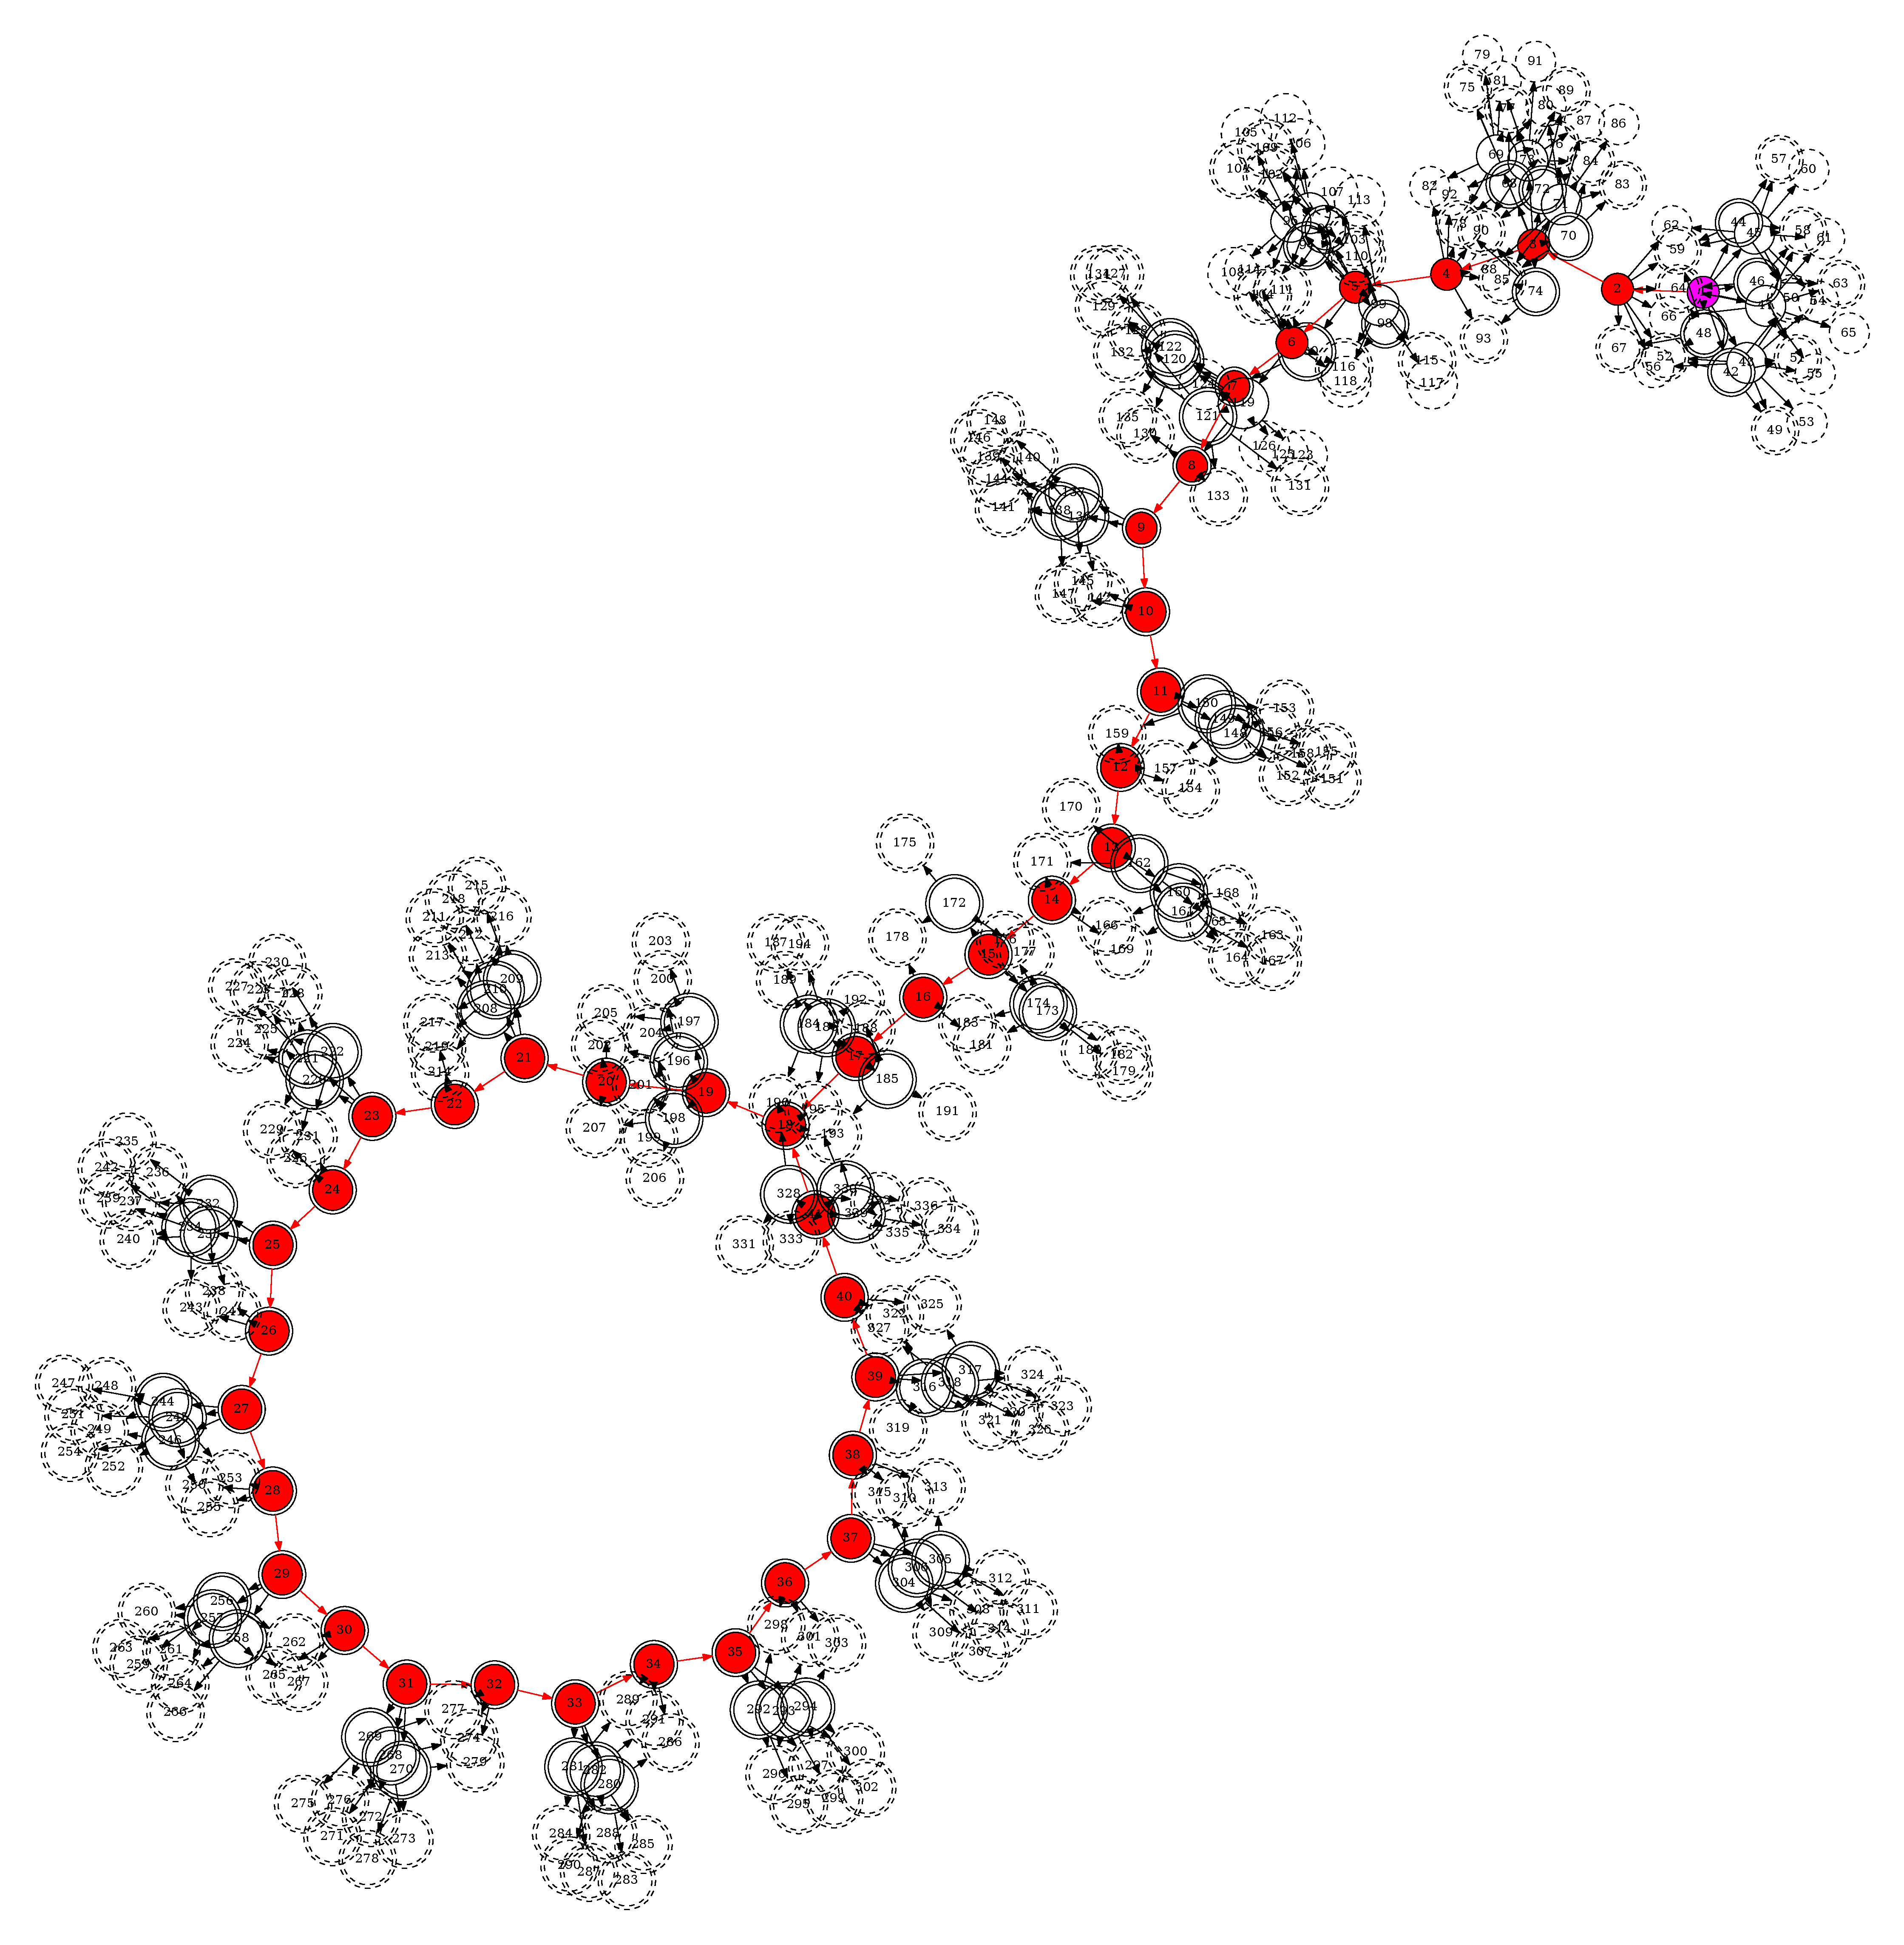
\includegraphics[width=.8\textwidth]{overview-neato.pdf}
}

\frame{\frametitle{/r/ModelCheckingPorn\hfill\#2}
\texttt{\small \$ divine draw examples/coffee.coin --labels -o coffee.pdf} \\
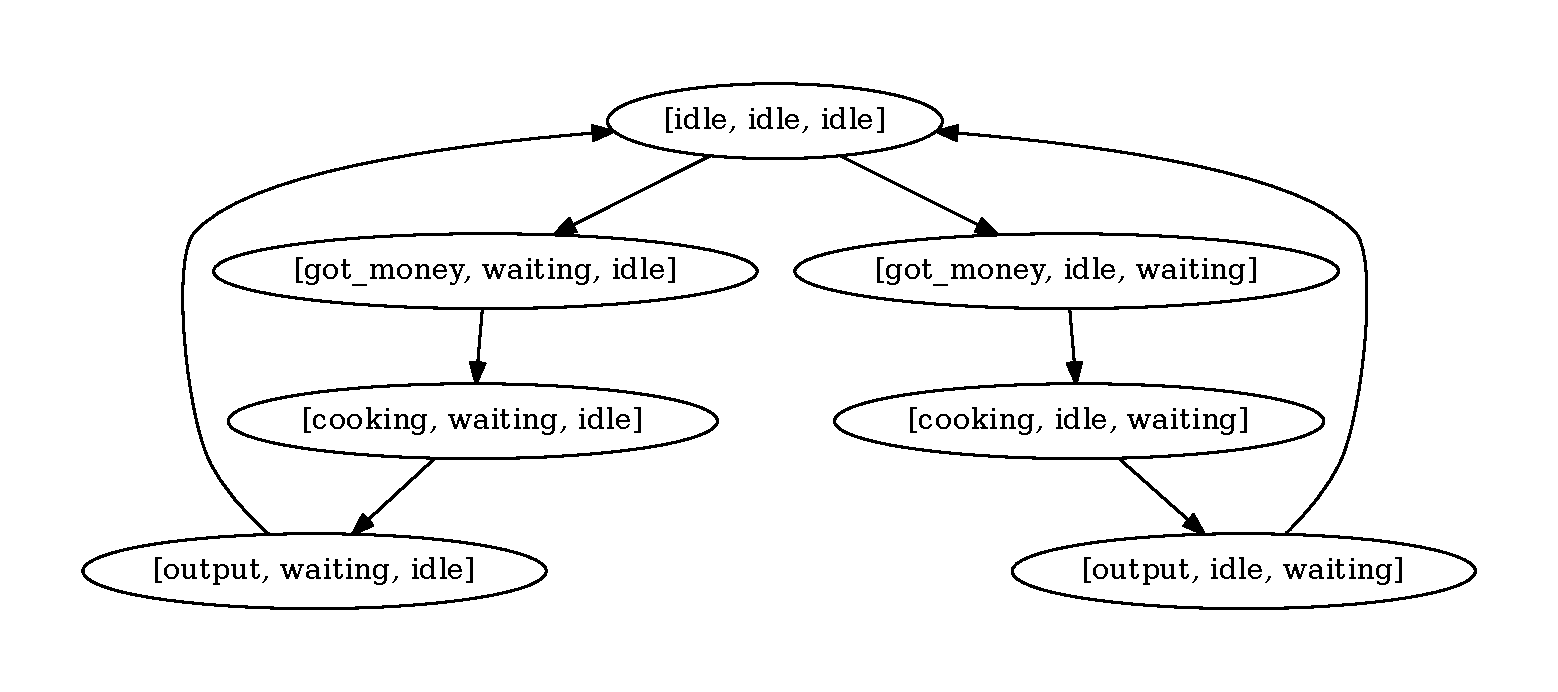
\includegraphics[width=\textwidth]{overview-coffee.pdf}
}



\frame{\frametitle{divine.simulate [OBSOLETE]}
\textbf{Purpose}
\begin{itemize}
\item Quick simulation of DVE systems in text console.
\item Can simulate traces (counterexamples).
\end{itemize}
\bigskip
\textbf{Problem}
\begin{itemize}
\item Comes from \divine Cluster.
\item Traces as produced by \divine 2.x are incompatible.
\end{itemize}

\bigskip

$\Rightarrow$ just use the GUI, or divine draw
}


\frame{\frametitle{GUI}
\textbf{Availability}
\begin{itemize}
\item Needs QT $>= 4.5$ to compile.
\item Available as separate binary, \texttt{divine.ide}.
\end{itemize}
\bigskip
\textbf{Features/Restrictions}
\begin{itemize}
\item Text editor for DVE systems.
\item Simulator/debugger for DVE system traces (counterexamples).
\item LTL property specification via plain text.
\item Executes only shared-memory verification tasks.
\end{itemize}
}




% BEWARE! compile outputs to the working directory!

\frame{\frametitle{Examples within bundle}
\textbf{Where}
\begin{itemize}
\item divine-2.5.2/examples/
\end{itemize}
\bigskip

\textbf{Example models}
\begin{itemize}
\item A few \texttt{.dve} models.
\item \texttt{cashier.prop2.coin}
\end{itemize}  
\bigskip
\textbf{CESMI}
\begin{itemize}
\item \texttt{circuit.h, circuit.cpp} \hfill Dataflow interface
\item \texttt{Data/* Divine/* Benchmark.hs} \hfill Haskell interface
\item \texttt{BenchmarkC.c} \hfill C interface
\end{itemize}
}


\frame{\frametitle{Input modelling languages}

\textbf{Native language(s)}
\begin{itemize}
\item DVE
\item CoIn (Component Interaction Automata)
\item LLVM [NOT IN 2.5]
\end{itemize}
\bigskip
\textbf{Other languages}
\begin{itemize}
\item ProMeLa (Protocol Meta Language, SPIN), supported through legacy NIPS-VM integration
\end{itemize}
\bigskip
\textbf{Binary interface (CESMI)}
\begin{itemize}
\item Compiled DVE
\item Mur$\varphi$
\item Dataflow Programs (through \texttt{circuit.h})
\item C and Haskell interfaces
\end{itemize}
}


\begin{frame}[fragile]
 \frametitle{Verifying Mur$\varphi$, ProMeLa}
\textbf{Mur$\varphi$}
\begin{verbatim}
$ divine compile sci.m
$ divine reachability sci.m.so
(...)
\end{verbatim}

\textbf{ProMeLa}
\begin{verbatim}
$ divine.compile-pml example.pm
$ divine metrics example.pm.b
  exploring... 			 done
 =====================================
         901 states
        1995 transitions
           0 accepting
          16 deadlocks
 =====================================
\end{verbatim}
\end{frame}

\frame{\frametitle{Input/Feature table}
  \footnotesize
  \renewcommand{\arraystretch}{1.3}
  \hspace*{-1.5em}
  \begin{tabular}{r|c@{\hskip.7em}c@{\hskip.7em}c@{\hskip.7em}c@{\hskip.7em}c@{\hskip.7em}c@{\hskip.7em}c@{\hskip.7em}c}
    \hline
      & DVE & DVE' & Mur$\varphi$ & CESMI & CoIn  & ProMeLa & compact & LLVM\footnote{NOT IN 2.5} \\
   \hline
   metrics & + & + & + & + & + & + & + & + \\
   deadlocks & + & + & + & + & + & + & + & + \\
   assertions & -- & -- & -- & -- & -- & -- & -- & + \\
   LTL & + & + & --  & + & + & 1/2 & + & + \\
   fairness\footnote{weak fairness + LTL} & -- & + & -- & --  & -- & -- & n/a & -- \\
   POR &-- &+ & -- & -- & + & -- & n/a & 1/2 \\
   symmetry & -- & -- & +  & n/a & -- & -- & n/a & -- \\
   simulator & + & -- & --  & n/a & -- & -- & -- & + \\
   \hline
  \end{tabular}

}


\frame{\frametitle{Beyond 2.5.2}
  \begin{itemize}
  \item Verification of LLVM bitcode (C, C++ \& more)
  \item Hash compaction (lossy compression). %[Jan Havlíček]
  \item (Loss-less) state compression.
  \item LTL MC of models with real-time via region abstraction. %[T. Janoušek]
  \item Better POR for reachability.
  \item Trading space for time.
  \item Symbolic algorithms against data explosion.
  \item Synchronous DVE.
  \item CESMI extensions (POR, system type identification)
  \item Slicing with respect to verified property for DVE and LLVM bitcode,
    COIN, ...
  \end{itemize}
}

\begin{frame}[fragile]
  \frametitle{Appendix 1: LLVM}

    Goal: Direct model checking of C \& C++ code. \\
    $\Rightarrow$ LLVM IR (Intermediate Representation; BitCode)

  \bigskip

  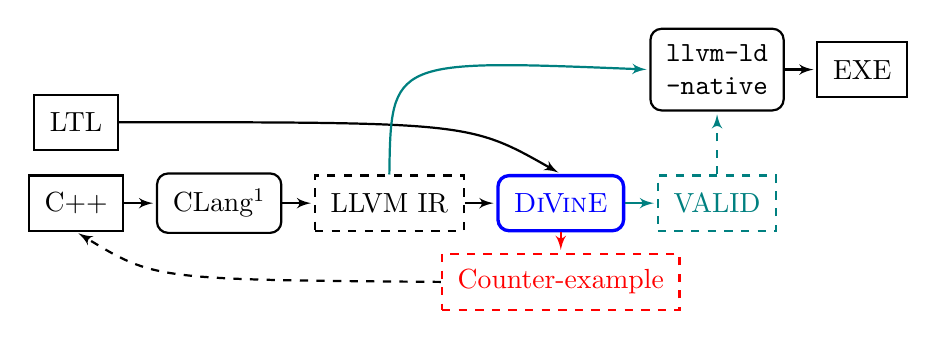
\begin{tikzpicture}
    \tikzset{
      box/.style={rectangle,draw=black, inner sep=2mm, minimum size=7mm, text centered,thick},
      tool/.style={rectangle,rounded corners,draw=black, thick, inner sep=2mm, minimum size=7mm, text centered},
      tool!/.style={rectangle,rounded corners,draw=black, very thick, inner sep=2mm, minimum size=7mm, text centered,blue},
      arrow/.style={->, >=latex', shorten >=1pt, thick}
    }


    \node[box] (LTL) {LTL};
    \node[box,below=3mm of LTL] (C) {C++};

    \node[tool,right=4mm of C] (CLANG) {CLang\footnote{Alternatively, GCC +
        dragonegg}};
    \node[box,dashed,right=4mm of CLANG] (BC) {LLVM IR};
    \node[tool!,right=4mm of BC] (DIVINE) {\divine};

    \draw[arrow] (LTL.east) .. controls (5,0) .. (DIVINE.north);
    \draw[arrow] (BC.east) -> (DIVINE.west);

    \draw[arrow] (C.east) -> (CLANG.west);
    \draw[arrow] (CLANG.east) -> (BC.west);

    \node[box,dashed,red,below of=DIVINE] (CE) {Counter-example};
    \draw[arrow,red] (DIVINE.south) -> (CE.north);
    \draw[arrow,dashed] (CE.west) .. controls (1,-2) .. (C.south);

    \node[box,dashed,right=4mm of DIVINE,teal] (OK) {VALID};
    \draw[arrow,teal] (DIVINE.east) -> (OK.west);

    \node[right=30mm of LTL] (XX) {};
    \node[tool,above=8mm of OK] (LLVM) {\texttt{\vbox{\hbox{llvm-ld}\hbox{-native}}}};

    \draw[arrow,teal,dashed] (OK.north) -> (LLVM.south);
    \draw[arrow,teal] (BC.north) .. controls (4,0.8) .. (LLVM.west);

    \node[box,right=4mm of LLVM] (EXE) {EXE};
    \draw[arrow] (LLVM.east) -> (EXE.west);

  \end{tikzpicture}
\end{frame}

\begin{frame}[fragile]
  \tiny
\begin{verbatim}
 1: #include "divine-llvm.h"
 2: 
 3: struct state {
 4:     volatile int flag[2];
 5:     int turn;
 6:     volatile int in_critical[2];
 7: };
14: 
16: void thread( struct p *p ) {
17:     p->s->flag[p->id] = 0; // BUG. Should assign 1 here.
18:     p->s->turn = 1 - p->id;
19:     while ( p->s->flag[1 - p->id] == 1 && p->s->turn == 1 - p->id ) ;
20:     p->s->in_critical[p->id] = 1;
21:     trace("Thread %d in critical.", p->id);
22:     assert( !p->s->in_critical[1 - p->id] );
23:     p->s->in_critical[p->id] = 0;
24:     p->s->flag[p->id] = 0;
25: }
26: 
27: int main() {
28:     struct state *s = malloc( sizeof( struct state ) );
29:     struct p *one = malloc( sizeof( struct p ) ),
20:              *two = malloc( sizeof( struct p ) );
31:     if (!s || !one || !two)
32:         return 1;
33: 
34:     one->s = two->s = s;
35:     one->id = 0;
36:     two->id = 1;
37: 
42:     pthread_create( &one->ptid, NULL, thread, one );
43:     pthread_create( &two->ptid, NULL, thread, two );
44:     pthread_join( one->ptid, NULL );
45:     pthread_join( two->ptid, NULL );
46:     return 0;
47: }
\end{verbatim}
\end{frame}

\begin{frame}[fragile]
\tiny
\begin{verbatim}
===== Trace from initial =====

[ peterson.c:29 ]

[ peterson.c:42 ]

[ divine-llvm.h:54 ]
[ divine-llvm.h:57 ]
[ divine-llvm.h:53 ]

[ divine-llvm.h:54 ]
[ peterson.c:19, p = *0x800 { 0, 0, *0x400 { [ 0, 0 ], 1, [ 0, 0 ] } } ]
[ divine-llvm.h:53 ]

[ divine-llvm.h:54 ]
[ peterson.c:20, p = *0x800 { 0, 0, *0x400 { [ 0, 0 ], 1, [ 1, 0 ] } } ]
[ divine-llvm.h:53 ]

[ divine-llvm.h:54 ]
[ peterson.c:22, p = *0x800 { 0, 0, *0x400 { [ 0, 0 ], 1, [ 1, 0 ] } } ]
[ peterson.c:18, p = *0x80c { 1, 1, *0x400 <...> } ]

[ divine-llvm.h:54 ]
[ peterson.c:22, p = *0x800 { 0, 0, *0x400 { [ 0, 0 ], 0, [ 1, 0 ] } } ]
[ peterson.c:19, p = *0x80c { 1, 1, *0x400 <...> } ]

[ divine-llvm.h:54 ]
[ peterson.c:22, p = *0x800 { 0, 0, *0x400 { [ 0, 0 ], 0, [ 1, 0 ] } } ]
[ peterson.c:20, p = *0x80c { 1, 1, *0x400 <...> } ]

===== The goal =====

[ divine-llvm.h:54 ]
[ peterson.c:22, p = *0x800 { 0, 0, *0x400 { [ 0, 0 ], 0, [ 1, 1 ] } } ]
[ peterson.c:20, p = *0x80c { 1, 1, *0x400 <...> } ]
! ASSERTION FAILED
\end{verbatim}
\end{frame}

\begin{frame}[fragile]
  \frametitle{Appendix 2: Probabilistic Model Checking}
  \begin{itemize}
    \item Not in 2.5.
    \item A new implementation of a distributed, OBF-based algorithm for
      probabilistic model checking has been merged recently. Work done by Jiří
      Appl as part of his diploma thesis. Will be part of \divine 2.6.
  \end{itemize}
\end{frame}

\end{document}

% LocalWords:  DiVinE LTL Checker Automata DFS DARCS darcs POSIX cmake
